  

\chapter{Deriving The Hubbard Model}

\section{Iridates}
% proper definition of iridates in section above
Iridium is a noble metal and one of the least common metals on earth and 
its density is among the highest among non-radioactive elements.
With an atomic number of 77 it is a transition metal of the platinum group.
Transition metals are characterized by a partially filled $d$-shell , which dominates their chemical behaviour.
As part of the heavier elements in the platinum group the $d$ orbitals belong to the 5th shell. 
Like many transition metals its $s$-shell of the next atomic number, the $6s$-shell, is filled as well.
In the atomic configuration the shell structure is $[\mathrm{Xe}]4f^{14}5d^7 6s^2$.
% ${\mathrm{Sr}}_{2}{\mathrm{IrO}}_{4}$
In compunds it can be found in different oxidation states, ranging from -3 to +6.
In the compounds treated in this thesis iridium is fourfold oxidized to $\mathrm{Ir}^{4+}$, 
which removes the $6s^2$ electrons as well as two electrons from the $5d$ shell.
The outermost shell is therefore the $5d$ shell, which is half-filled ~\cite{Abragam70}.


%(the ion shell structure does not follow the Aufbau principle. 
%Therefore has $\mathrm{Ir}^{4+}$ a different shell structure than Tantalum, even though they have the same number of electrons. 
%This is because of the different charge of the nucleus, that leads to a greater seperation in energs levels with different quantum number n ($\propto \frac{Z}{n^2}$)).

The other elements of the compounds treated in this thesis are oxygen and rare earth metals. 
The oxygen is two fold ionized and has therefore only the closed shells $1s^2,2s^2,2p^6$.
The same hold for the rare earth metals, strontium is reduced to 
$\mathrm{Sr}^{2+}$ with the electron configuration of $\mathrm{Kr}$. 
Both the rare earth metal and oxygen have therefore zero total angular momentum and spin. 

Iridates show a great variety of geometrical configurations. 
We will focus on Sr$_2$IrO$_4$, which is part of the Ruddelson-Popper series of Iridium oxides, Sr$_{n+1}$Ir$_{n}$O$_{3n+1}$ with $n =1$. 
$n$ counts the layers of perovskite structure that are stacked directly on top of each other, 
before being separated by Sr ions. 
Other possible values in this series are 2 and $\infty$, where the last one means there is no separation anymore and we have SrIrO$_3$. 
Sr$_2$IrO$_4$ has the structure of a layered perovskite, that means it consists of single layers with a structure similar to CaTiO$_3$.
The later one is also called perovskite and lends its name to the perovskite structure.
It consists of a cubic unit cell, with one type of atom (Ca in perovskite) on the edges, 
the  atom of the other element (Ti) is embedded in an octahedron of 
oxygen ions, which are located on the face centers, see figure \ref{pervoskite} for an illustration.
%
% picture perovskite unit cell
\begin{figure}[!htbp]
 \centering
 \includegraphics[width=.5\textwidth]{../Image_Perovskite}
 \caption{Unit cell of a perovskite, the building block of many iridates. The yellow dots represent the rare earth metal, the white dots form the octahedra of the oxygen ligands. The black dot is the iridium ion.
	  Picture taken from \cite{Perovskitebilde}.}
	  \label{perovskite}
\end{figure}
%
In the case of Sr$_2$IrO$_4$ it is Ir$^{4+}$ that is located  inside the octahedra. 
The type of rare earth metal as well as the ratio determine different geometrical setups of octahedra. 
They share corners only in the $x$-$y$-direction while beeing separated by a Sr$^{2+}$ ion in the z-direction.
Due to a shift between two subsequent layers, we have to include two layers in the unit cell in order to regain a cubic one.
An octahedron of one layer matches an Sr ion of the other, perventing  corner sharing in the $z$-direction and providing thereby the separation of layers. 
% 
Furthermore, the octahedra are tilted in a staggered pattern by $\Theta = \pm 11^{\circ}$ \cite{PhysRevB.49.9198}.
This enlarges the cubic unit cell to $\sqrt2 a\times\sqrt 2b \times 2c$.
In $x$- and $y$-direction we have to take two irdium ions into the unit cell. The translation vector corresponds now to the former diagonals.
At the same time we get 4 layers in $z$-direction, until the same pattern of tilted octahedra is met again. The unit cell is shown in figure \ref{unitcell}
%
\begin{figure}
\centering
\includegraphics[width=.7\textwidth]{../medium.png}
\caption{a) Tetragonal unit cell of \Sriro. \quad b) Two dimensional layers of perovskite structure \newline Figure taken from \cite{PhysRevLett.108.177003}.}
\label{unitcell}
\end{figure}
%
We will neglect the rotations in proceeding to an model of effective spins, but regain the influence it has on the magnetic structure in the final interpretation of 
response functions. It shows that these rotations provide an explanation for the small ferromagnetic moment in the otherwise antiferromagnetic material. 

\subsubsection{Ligand Field}

The $5d$ states  in a free iridium ion are degenerate due to rotational symmetry of the atomic Hamiltonian. 
We choose the cubic harmonics as a basis and  denote the states by according to their transformation symmetry with respect to the coordinat axes, namely 
$\ket{x^2-y^2},\ket{z^2},\ket{xy},\ket{xz}$ and $\ket{yz}$.
The cubic harmonics are related to the spherical harmonics  of the $d$-orbitals, $Y^2_m$ for $m=0,\pm1,\pm2$, by a unitarian transformation, shown in table \ref{sphericHarmonics}.
As such, the cubic harmonics have all angular momentum $l=2$. 
and they form an irreducible representation of the rotation group.
\begin{table}
\begin{center}
\begin{tabular}{|c|c|c|}
 \hline
 $xy$ & $\frac{\im}{\sqrt 2} \left( Y^{-2}_2 - Y^2_2 \right)$ & $\sqrt{\frac{15}{4\pi}} \frac{xy}{r^2}$ \\
 $xz$ & $\frac{  1}{\sqrt 2} \left( Y^{-1}_2 - Y^1_2 \right)$ & $\sqrt{\frac{15}{4\pi}} \frac{xz}{r^2}$ \\
 $yz$ & $\frac{\im}{\sqrt 2} \left( Y^{-1}_2 + Y^1_2 \right)$ & $\sqrt{\frac{15}{4\pi}} \frac{yz}{r^2}$ \\
 $z^2$& $ Y^0_{2} 					      $	& $\sqrt{\frac{15}{4\pi}} \frac{3z^2-r^2}{2r^2\sqrt 3} $\\
 $x^2-y^2$&$\frac1{\sqrt 2} \left( Y^{-2}_2 + Y^2_2 \right) $ & $\sqrt{\frac{15}{4\pi}} \frac{x^2-y^2}{2r^2} $ \\
 \hline
\end{tabular}
\caption{Definition of cubic harmonics of the $d$ orbitals and their relation to the spherical harmonics.}
\label{sphericHarmonics}
\end{center}
\end{table}
%

Embedding the iridium ion in a crystal breaks the rotational symmetry of the potential due to anisotropic contributions from its neighbours.
As a result, the degeneracy of the $5d$ states will be lifted. 
Since the ion is now surrounded by the ligands in the form of an octahedron, the 
full rotational symmetry is reduced to transformation symmetries of the octahedron or equally a cube. 
These are the 48 transformation of the point group $O_h$.
One can tell from group theory alone, that reducing the symmetry splits an irreducible representation of the rotational group into subgroups, that form irreducible representations 
corresponding to the lowered symmetry. 
Comparing the characters of the irreducible presentations for $O_h$ with the ones for the full rotational group SO(3), we find that 
the latter one has to split up into one  two dimensional and one three dimensional subgroup. 
The degeneracy of the $5d$ states is thereby partially lifted and we get the 
three-fold degenerate $t_{2g}$ states consisting of the $xy,xz,yz$ orbitals and the two-fold degenerate $e_g$ states formed by $z^2$ and $x^2-y^2$ \cite[Chapter~4]{Tinkham64} 

The value of the energetic split due to the crystal field depends on the form and strength of the potential generated by the ligands. 
In \Sriro it is of order $\Delta_c  = E(e_g) - E(t_{2g})\approx 5$eV \cite{PhysRevB.80.075112}. 
The sign is such that the $e_g$ states lie at a  higher energy than the $t_{2g}$,
which can be understand in an intuitive way from the form of the orbitals.
The $e_g$ states fill the space closer to the ligands, requiring therefore 
energy to overcome the repulsion from the negatively charged oxygen ions,
while the $t_{2g}$ orbitals avoid the ligands by being extended along the diagonals of the unit cell. 
% neglect stretching in z-direction and hybridization with e_g due to rotations
The orbitals are then not filled according to Hund's rule,
which decreases the inter-particle interaction by filling all orbitals with particles of the same spin,
before filling orbitals with two particles of opposite spin. 
The resulting spatially antisymmetric wave function reduces then the overlap of wavefunctions.

In the case of iridium we deal with  $5d$ states, which are more extended than the $4d$ and $3d$ states of lighter transition metals. 
This reduces the overall amplitude of the wavefunction and therefore  the repulsion between electrons on different sites. 
The energy split due to the crystal field is strong enough to favour double occupancies in the $t_{2g}$ states over populating the $e_g$ states. 
As a result, the $e_g$ states are empty, while all five electrons will be distributed over the $t_{2g}$ states. 





\section{Strong Spin-Orbit Coupling}


Until now we neglected interactions between angular momentum and spin. 
The coupling $\zeta_{\mathrm{SO}}$ of total angular momentum $L$ and total Spin $S$ is proportional to the charge of the nucleus to the 4th power, $Z^4$.
Spin orbit coupling (SOC) becomes therefore more important in heavier elements and is no longer negligible in iridates.
Strong SOC is the main difference between iridates and cuprates.
It is the cause of interesting new effects like the insulating behaviour up to high temperatures. 

The total effective angular momentum of the $t_{2g}$-states is $L=1$. 
There are five electrons in the three states, leaving one hole.
Due to the Pauli principle, only three electrons can have the same spin, 
the other two must have the opposite spin. 
The total spin $S$ adds therefore up to $\frac12$.
The total angular momentum and total spin can then be coupled to
$J=\frac32$ and $J=\frac12$.
%
SOC accounted for by adding the term $\zeta_{\mathrm{SO}} \sum_{i} \hat{\vec L} \cdot \hat{\vec S}$ to the Hamiltonian,
where $\zeta_{\mathrm{SO}}$ denotes the coupling strength. 
Its value in Sr$_2$IrO$_4$ is given by $\zeta_{\mathrm{SO}} = 0.37$eV \cite{PhysRevLett.105.216410}.

The matrix elements of the interaction term in the cubic harmonics basis are given by 
\begin{equation}
\bra{\alpha,\sigma} \hat{\vec L} \cdot \hat{\vec S} \ket{\beta,\sigma^{\prime}} = \sum_{j=x,y,z}\bra{\alpha} \hat L_j \ket{\beta} \bra{\sigma} \hat S_j \ket{\sigma^{\prime}} 
\end{equation}
with $\alpha, \beta \in \{xy,xz,zy\}$ and the spin values $\sigma, \sigma^{\prime} \in \{\uparrow,\downarrow\}$.
% notation of \sigma as number
The angular momentum matrix elements can be easily calculated by the substitution $L_x=\frac12 (L^++L^-)$ and $L_y=\frac{-\im}2 (L^+-L^-)$.
and expressing the $t_{2g}$-states through the spherical harmonics.
The components of the angular momentum operators act on the spherical harmonics through 
$L_z Y^m_l = m Y^m_l \:$, $L^+Y^m_l = \sqrt{(l-m)(l+m+1)}Y^{m+1}_l$ and $L^-Y^m_l = \sqrt{(l+m)(l-m+1)}Y^{m-1}_l$.
The spin operator is proportional to the Pauli matrices, $\tau_j = \frac12 \sigma_j$.
We are left with a hermitian matrix with only six independent, non-zero components, namely
\begin{IEEEeqnarray}{rCl}
 \bra{zx,\sigma} \hat{\vec L} \cdot \hat{\vec S} \ket{xy,-\sigma} &=& \frac{\im\zeta_{\mathrm{SO}}}2 \nonumber \\
 \bra{yz,\sigma} \hat{\vec L} \cdot \hat{\vec S} \ket{xy,-\sigma} &=& -s_{\sigma}\frac{\zeta_{\mathrm{SO}}}2 \nonumber \\
 \bra{zx,\sigma} \hat{\vec L} \cdot \hat{\vec S} \ket{zx,\sigma}  &=& s_{\sigma} \frac{\im \zeta_{\mathrm{SO}}}2,
\end{IEEEeqnarray}
where $s_{\uparrow}=+1$, $s_{\downarrow}=-1$ denote the signs of the spins.
This matrix has two eigenvalues, $-\nicefrac{\zeta_{\mathrm{SO}}}2$ and $+\zeta_{\mathrm{SO}}$. The subspace for the lower one is 4 dimensional and corresponds to 
the $J_{\mathrm{eff}}=\frac32$ state, the other one is the two-dimensional $J_{\mathrm{eff}}=\frac12$ subspace. 
In the ground state the $J=\frac32$ band will be completely occupied, while the $J=\frac12$ band is half-filled.
Figure \ref{split_states} shows the energetic split and the occupancy of energy levels in the ground state.
%
%for LS-coupling: 
%\cite{PhysRevLett.105.216410}
%
\begin{figure}
 \begin{center}
 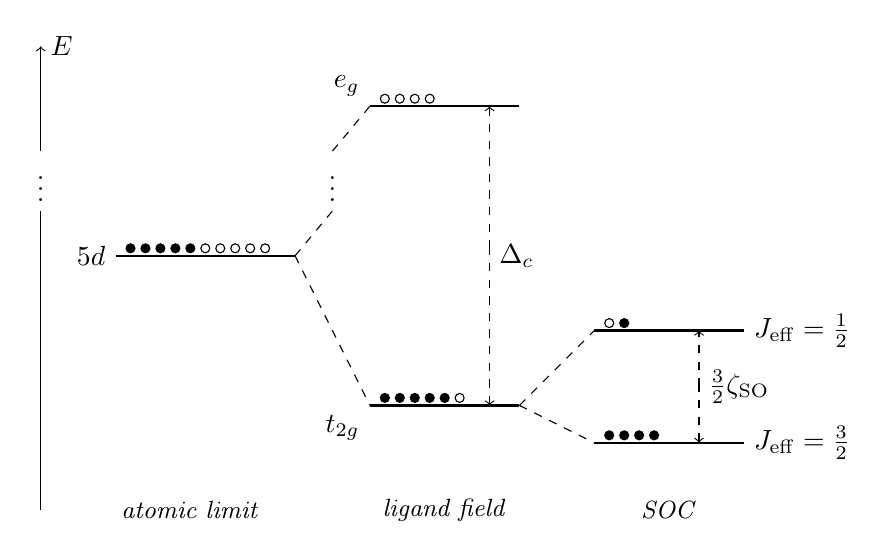
\begin{tikzpicture}[scale=1.9]
 \draw[-] (-0.7,.8) -- (-.7,2.8) node[anchor = south]{$\vdots$} ;
 \draw[->] (-0.7,3.2) -- (-.7,3.9)node[anchor =  west]{$E$};
 \draw[-,black  ,thick] (-0.2,2.5)node[anchor=east] {$5d$} -- (1.0,2.5);
 \foreach \f in {-0.1,0.0,...,0.4} \filldraw (\f,2.55) circle (0.03);
 \foreach \f in {0.4,0.5,...,0.9} \draw (\f,2.55) circle (0.03);
 %
 \draw[-,black,dashed] (1.0,2.5) -- (1.25,2.8) node[anchor= south]{$\vdots$};
 \draw[-,black,dashed] (1.25,3.2) -- (1.5,3.5);
 \draw[-,black,dashed] (1.0,2.5) -- (1.5,1.5);
 %
 \draw[-,black  ,thick] (1.5,3.5)node[anchor=south east] {$e_g$} -- (2.5,3.5);
  \foreach \f in {1.6,1.7,...,1.9} \draw (\f,3.55) circle (0.03);
 \draw[-,black  ,thick] (1.5,1.5)node[anchor=north east] {$t_{2g}$} -- (2.5,1.5);
  \foreach \f in {1.6,1.7,...,2.0} \filldraw (\f,1.55) circle (0.03);
  \draw (2.1,1.55) circle (0.03);
 %
 \draw[-,black,dashed] (2.5,1.5) -- (3,2.0);
 \draw[-,black,dashed] (2.5,1.5) -- (3,1.25);
 %
  \draw[-,black  ,thick] (3,2.0) -- (4,2.0) node[anchor= west] {$J_{\mathrm{eff}}=\frac12$} ;
  \draw (3.1,2.05) circle(0.03);
  \filldraw (3.2,2.05) circle(0.03);
 \draw[-,black  ,thick] (3,1.25) -- (4,1.25) node[anchor= west] {$J_{\mathrm{eff}}=\frac32$};
  \foreach \f in {3.1,3.2,...,3.4} \filldraw (\f,1.3) circle (0.03);
  % energie differences
  \draw[<-,black, dashed] (3.7,1.25) -- (3.7,1.625) node[anchor = west]{$\frac32\zeta_{\mathrm{SO}}$};
  \draw[->,black, dashed] (3.7,1.625) -- (3.7,2);
  %
  \draw[<-,black, dashed] (2.3,3.5) -- (2.3,2.5) node[anchor = west]{$\Delta_c$};
  \draw[<-,black, dashed] (2.3,1.5) -- (2.3,2.6);
  %
  \draw (0.3,0.8) node[]{\small{\emph{atomic limit}}};
  \draw (2.0,0.8) node[]{\small{\emph{ligand field}}};
  \draw (3.5,0.8) node[]{\small{\emph{SOC}}};
 \end{tikzpicture}
\caption{scheme of the split-up of states due to the crystal field and spin orbit coupling. The circles indicate the available spaces and are filled if occupied.}
 \label{split_states}
\end{center}
\end{figure}

%
The two eigenstates of $J_{\mathrm{eff}}=\frac12$ are given by a linear combination of the molecular orbitals and spin states,
\begin{equation}
 \ket{J_{\mathrm{eff}} =\frac12, M_{J_{\mathrm{eff}}}= \sigma}
 = 
 \frac{1}{\sqrt{3}} \left( \ket{yz,\sigma} -s_{\sigma} \im \ket{zx,\sigma} -s_{\sigma} \ket{xy,-\sigma} \right).
\end{equation}
%\todo{transformation properties of the ground state}
% possible: construct J_eff first (3/2 and 5/2, the second splitting up to 1/2 and 
%%%%%%%%%%%%%%%%%%%%%%%%%%%%%%%%%%%%%%%%%%%%%%%%%%%%%%%%%%%%%%%%%%%%%%%%%%%%%%%%%%%%%%%%%%%%%%%%%%%%%%%%%%%%%%%%%%%%%%%%%%%%%%%%%%%%%%%%%%%%%%%%%%%%%%%%%%%%%%%%%%%%%%%




%\subsubsection{Relative Orientation Of Octahedra}
% rotation by 11° in Sr$_2$IrO$_4$, corner sharing
% edge sharing in other materials, non 2D setup

\newpage
\section{The Hubbard Model}

So far we considered only ions and their immediate vicinity in the limit of infinite separation from each other, 
i.e. without the influence of a crystal pattern and interactions between different sites of the lattice.
In reality the orbitals constructed above show some overlap, which creates the possibility of transitions and interactions between neighbouring sites.
In this chapter we show, that it is possible to construct a set of localized orthonormal states based on atomic states. 
This allows us then to describe the system using second quantization.


\subsection{Tight Binding Model} % in second quantization

Electrons in iridates are localized, i.e. they are well described by wave functions
which are centred around sites in the crystal and fall off fast as one is moving further away. 
Atomic orbitals provide a good starting point for this case.
%Since we are interested in dynamics at low temperatures we restrict ourself to the $J=\frac12$ orbital, that is situated at the Fermi level. 
%Other orbitals are either completely filled or well above the Fermi level and therefore not important in the dynamics of the system at low temperatures.


We denote the $n$th orbital of the unit cell at site $\vec R_i$ with $\ket{\phi_I} = \phi^n(\vec r - \vec R_i)$.
$I=(n,i)$ is the combined index of orbital number $n$ and site number $i$. $n$ runs over the relevant orbitals of all atoms in the unit cell. 
%
Even though the orbitals are localized, we have a non-zero overlap for different $I=(i,n)$ and $J=(j,m)$, $\braket{\phi_I}{\phi_J} = S_{IJ}\ne \delta_{IJ}$.
This includes overlaps in the unit cell and across sites. 
%
The potential in the Hamiltonian is now the sum over atomic potentials at all sites, and the total single-particle Hamiltonian reads
\begin{IEEEeqnarray}{rCl}
 \hat H &=& \frac{1}{2m}\nabla^2 - \sum_I V^n_{\mathrm{atom}}(\vec r - \vec R_i ) \nonumber \\
 &=& H_{\mathrm{atom}}^n(\vec R_i) - \sum_{J\ne I} V^m_{\mathrm{atom}}(\vec r - \vec R_j )
\end{IEEEeqnarray}
In the last line we grouped the terms belonging to the single atom Hamiltonian at space $\vec R_i$, of which $\ket{\phi_I}$ is an eigenfunction with eigenvalue $E^n$.
This allows us to easily identify different contributions the matrix elements of the Hamiltonian.
\begin{equation}
 \bra{ \phi_I} \hat H \ket{\phi_J} = E^{n}\mathbf S_{IJ}-\beta^{m}\delta_{IJ} - \mathbf T_{IJ}
\end{equation}
$\beta^m$ corresponds to a shift of energy, due to the integral over the atomic potentials located on all sites apart $I$,
\begin{equation}
 \beta^m = \int \!\!\dint^3 r \:\: \phi^n(\vec r - \vec R_i)^* \sum_{I^{\prime}\ne I} V^{n^{\prime}}_{\mathrm{atom}}(\vec r - \vec R_{i^{\prime}} ) \phi^n(\vec r - \vec R_i)
\end{equation}
This contribution will be small, since $\phi^n(\vec r-\vec R_i )$ is small outside the unit cell at $\vec R_i$.
The matrix $\mathbf T_{IJ}$ consists of all non-diagonal integrals of this type, 
\begin{equation}
 \mathbf T_{IJ} = \int \!\!\dint^3 r\:   \: \phi^{n*}(\vec r - \vec R_i) \sum_{I^{\prime}\ne I} V^{n^{\prime}}_{\mathrm{atom}}(\vec r - \vec R_{i^{\prime}} ) \phi^m(\vec r - \vec R_j)
\end{equation}
if $I \ne J$ and 0 otherwise. 
The biggest contribution in the sum comes from the term with $I^{\prime}=J$, since one wave function has a central overlap with the potential.

We want to transform our basis states such that they are orthonormal but still located around lattice sites.
Functions of this type are the Wannier functions $\Psi_I$. They are given by the Fourier transformation of Bloch functions.
We introduce a combined index for $k$-space as well, $K=(n,\vec k)$.
Changing to Fourier space is a unitary operation that can be expressed in matrix notation.
The transformation matrix $\mathbf{U}$ is defined through 
$
 \mathbf{U}_{IK} = N^{-\frac12} \euler^{\im\vec k \vec R_i} \delta_{nm}.
$ and we can write
\begin{equation}
 \Psi_I \left( \vec{r} \right) = \frac1{\sqrt{N}} \sum_{\vec{k}} \euler^{\im \vec{k}\vec{R}_i } \Psi_K(\vec r) = \sum_{K} \mathbf{U}_{IK} \Psi_K(\vec r) 
\end{equation}
%
Bloch functions are eigenfunctions of the translation operator of the lattice. 
Under a symmetry translation of the lattice, they will only pick up a phase,
\begin{equation}
 \Psi_{K} \left( \vec{r}+\vec{T}\right) = \euler^{\im \vec{k} \vec{T} } u_{K} \left( \vec{r} \right). \label{BlochDef}
\end{equation}
$\vec T$ is a translation vector of the lattice and $u_{K} \left( \vec{r} \right)$ is a function with the same periodicity as the lattice. 
As eigenfunctions the Bloch states are orthogonal, 
which can also be seen by the completeness relation of $\sum_i \euler^{\im ( \vec k - \vec k^{\prime} ) \vec R_i} = N\delta (\vec k - \vec k^{\prime})$
Since the transformation to Wannier states is a unitary transformation, e.g. $\mathbf U^{\dagger} = \mathbf U^{-1}$, it follows immediately that they are orthogonal as well.

We can now construct Bloch functions from the atomic functions by means of Bloch sums.
\begin{equation}
  \Psi_K(\vec{r}) = N_K \sum_{i} \euler^{\im \vec{k}\vec{R}_i }  \phi^n(\vec{r}-\vec{R}_i). 
\end{equation}
$N_K$ is a $k$- and $n$-dependent normalization factor
\begin{IEEEeqnarray}{rCl}
 N_K^{-2}  &=&  \sum_{i,j} \euler^{\im \vec k (\vec R_i-\vec R_j)}   
 \int \!\! \dint^3 r {\phi^n}^*(\vec r - \vec R_i) \phi^n(\vec r- \vec R_j) 
 \nonumber \\ &=& 
 \sum_{IJ} \mathbf U^{\dagger}_{KI} S_{IJ} \mathbf U_{JK}
\end{IEEEeqnarray}
Constructed in this way, the states fulfil the requirement of \ref{BlochDef}, since
\begin{IEEEeqnarray}{rCl}
 \Psi_{K}(\vec{r}+\vec{T}) 
 &=& N_{K} \euler^{\im \vec{k} \vec{T} } \sum_{i} \euler^{\im \vec{k} (\vec{R}_i-\vec{T})} \phi^n (\vec{r}-\vec{R}_i+\vec{T}) \nonumber \\
 &=& N_{K} \euler^{\im \vec{k} \vec{T} } \sum_{i} \euler^{\im \vec{k}\vec{R}_i }  \phi^{n}(\vec{r}-\vec{R}_i), 
\end{IEEEeqnarray}
where the second step is simply done by a shift in the sum. 
Using the Bloch sums to construct Wannier functions yields the states we are looking for.
These so called Löwdin orbitals are given by
\begin{equation}
 \ket{\varphi_I} = \sum_{j}  \sum_{\vec k} \euler^{\im \vec k ( \vec R_i - \vec R_j ) } N_k \ket{\phi_J}\delta_{mn}
 = \sum_{J} \left( \mathbf U(\mathbf U^*\mathbf S\mathbf U)^{-\frac12}\mathbf U^*\right)_{IJ} \ket{\phi_J}\delta_{mn} 
\end{equation}
Finally, we can express the Löwdin states in term of atomic orbitals and their overlaps,
\begin{equation}
 \ket{\varphi_I} = \sum_J (\mathbf S^{-\frac12})_{IJ} \ket{\phi_J}\delta_{mn}.
\end{equation}
The matrix $\mathbf S^{-\frac12}$ is defined by a Taylor series of the matrix $\mathbf S$. 
Therefore commute $\mathbf S$ and its square root and it follows that$\mathbf S^{-\frac12}$ is hermitian as well.
Since we have only small off-diagonal elements and 1 on the diagonal, we see that the Löwdin states are still
localized around the centres. 
In the limit of large separations, $\mathbf S$ approaches the identity, and we regain the atomic orbitals.
The main difference between the Löwdin states and the atomic ones are oscillations of the phase, that ensure orthogonality.


We can now express the matrix elements of the Hamiltonian in the new basis.
\begin{IEEEeqnarray}{rCl}
 \bra{ \varphi_I} \hat H \ket{\varphi_J} &=& (E^m-\beta^m)\delta_{IJ} - t_{IJ} \\
 t_{IJ} &=& \left\{ 
 \begin{array}{c@{\quad}l}
 -\beta \mathbf S_{IJ} - (\mathbf{S}^{-\frac12}\mathbf T \mathbf S^{-\frac12})_{IJ} & I \ne J \\
 0 & I=J 
 \end{array} \right. \nonumber 
\end{IEEEeqnarray}
%
The calculation of $t_{IJ}$ requires detailed knowledge about the atomic states and the periodic potential.
They are usually calculated through other approximation schemes, for example the local density approximation (LDA).
In calculations we will use values from the literature, that were fitted to LDA + SO calculations.


\subsubsection{Superexchange}
% and how spin exchanges happen 

The direct hopping terms between iridium orbitals are negligible, since the iridium sites are separated by oxygen ions
and the overlaps of orbitals from two different iridium atoms are negligible.
Transitions between iridium sites are still possible, when they are mediated through the $p$-orbitals of oxygen ions. 
These two step hopping processes are called super exchange and give rise to an anti-ferromagnetic coupling.
We will just sketch how to calculate the main contribution to an effective Ir-Ir hopping.

The oxygen ion  between two iridium atoms has completely filled $p$-orbitals, one of which is aligned 
along the line connecting the two iridium sites. 
Hopping to and from this orbital gives the most important contribution, while transitions between $p$-orbitals are forbidden.
We denote the parameter for hopping from an iridium orbital to the oxygen orbital by $t_p$. 
A scheme of the processes leading to super exchange can be seen in figure \ref{superexchange}.
%
\begin{figure}
\begin{center}
\begin{tabular}{c}
  
\begin{tikzpicture}
 \draw[-,thick] (0,0) -- (2,0);
 \draw[-,thick] (4,0) node[anchor = north west ]{$p$} -- (6,0) ;
 \draw[-,thick] (8,0) -- (10,0);
 %
 \draw[->,thick] (.8,-.5) -- (.8,.5);
 %
 \draw[->,thick] (4.8,-.5) -- (4.8,.5);
 \draw[<-,thick] (5.2,-.5) -- (5.2,.5);
 %
 \draw[->,thick] (9,-.5) -- (9,.5);
 %
 \draw[->,dashed] (5.2,.6) .. controls (4.2,1.3) and (2.2,1.3) .. node[above]{1.} (1.2,.6) ;
\end{tikzpicture}
\\
 
\begin{tikzpicture}
 \draw[-,thick] (0,0) -- (2,0);
 \draw[-,thick] (4,0) node[anchor = north west ]{$p$} -- (6,0) ;
 \draw[-,thick] (8,0) -- (10,0);
 %
 \draw[->,thick] (.8,-.5) -- (.8,.5);
 \draw[<-,thick] (1.2,-.5) -- (1.2,.5);
 %
 \draw[->,thick] (4.8,-.5) -- (4.8,.5);
 %
 \draw[->,thick] (9,-.5) -- (9,.5);
 %
 \draw[->,dashed] (9,.6) .. controls (8.2,1.3) and (6.2,1.3) .. node[above]{2.} (5.2,.6) ;
\end{tikzpicture}
\\ \\
\begin{tikzpicture}
 \draw[-,thick] (0,0) -- (2,0);
 \draw[-,thick] (4,0) node[anchor = north west ]{$p$} -- (6,0) ;
 \draw[-,thick] (8,0) -- (10,0);
 %
 \draw[->,thick] (.8,-.5) -- (.8,.5);
 \draw[<-,thick] (1.2,-.5) -- (1.2,.5);
 %
 \draw[->,thick] (4.8,-.5) -- (4.8,.5);
 \draw[<-,thick] (5.2,-.5) -- (5.2,.5);
\end{tikzpicture}
\end{tabular}
 \caption{scheme of the two processes involved in superexchange hopping between two iridium sites, mediated through a $p$-orbital from the ligands}
 \label{superexchange}
 \end{center}
\end{figure}
%
%
Since this involves two hopping processes, to and from the $p$-orbital, we get two  factors of $t_p$.
Projecting the oxygen states out leads to an additional factor of $\frac1E$ where $E=U+(E_d-E_p)$ is the energy of the intermediate step,
given by the energies of the $p$ and $d$ states plus an energy due to the repulsion between two electrons in the $d$ orbital. 
The effective hopping is then $t=\frac{t_p^2}{U+E_d-E_p}$.

%The diagonal term is still given by the eigenvalues of the atomic Hamiltonian with a shift due to the presence of the other potentials. 
%Since this term is proportional to unity, we can remove this factor from the Hamiltonian by shifting the energy scale.

\subsection{Second Quantization}

Having defined our single particle Hamiltonian in terms of orthonormal wave orbitals, 
we can construct the many particle wave function in terms of creation and annihilation operators. 
The operator $c^{\dagger}_{i,\sigma}$ creates a particle with spin $\sigma$ in the orbital $\ket{\varphi_i}$,
while its hermitian conjugate $c_{i,\dagger}$ removes it.
They have to fulfil the anti-commutation rules for fermions,
\begin{IEEEeqnarray}{rClrCl}
 \Big\{c^{\dagger}_{i,\sigma}\:,\: c_{j,\sigma^{\prime}} \Big\} &=& \delta_{ij} \delta_{\sigma, \sigma^{\prime}} 
 &\qquad
 \Big\{c_{i,\sigma}\:,\: c_{j,\sigma^{\prime}} \Big\} &=& 0 \nonumber \\
 \Big\{c_{i,\sigma}^{\dagger}\:,\: c^{\dagger}_{j,\sigma^{\prime}} \Big\} &=& 0 &&& \label{acomm_rules}
\end{IEEEeqnarray}
It follows immediately that  $-c^{\dagger}_{i,\sigma} c^{\dagger}_{j,\sigma} = c^{\dagger}_{j,\sigma} c^{\dagger}_{i,\sigma}$ and $(c^{\dagger}_{i,\sigma})^2 = 0$.
These relations ensure the antisymmetry of the total wave function and thereby the Pauli principle.


% looks like the same thing, but results in oscillations  at the overlapping tails, providing ON.
% Overlap integrals are transformed with that, providing then t_ij
% provides U_ijkl as well?
% see Altmann pp. 177 and 222

%Furthermore they are localized around the positions $\vec{R}_i$.
%Instead of the eigenfunctions of the single particle Hamiltonian, we can use linear combinations of them. 
%This gives us a different set of Wannier functions, that are related to the ones previously defined by another unitary transformation.
%The additional degrees of freedom can be used to optimize the Wannier functions according to certain criteria.
%The most common ones are maximal localization or symmetries of the crystal or the atomic orbitals.
% By taking a relevant subset of atomic states, and defining for each $\vec{k}$
%\begin{equation}
% H_{nm} = \bra{\Psi_{n,\vec{k}}} H \ket{\Psi_{m,\vec{k}}} \text{  and  } S_{nm} = \braket{\Psi_{n,\vec{k}}}{\Psi_{m,\vec{k}}}
%\end{equation}
%we can set up the secular equation
%\begin{equation}
% \det(H_{nm}-E_kS_{nm})=0.
%\end{equation}
%This gives us the band energies. The corresponding eigenstates are called Löwedin functions.
% BAD writing here, tsss. What is the poinit anyway?
% resemble the Löwedin states the crystal symmetry? They should (--> see Slater et al.)



%In this picture we think of electrons as being in a certain state of an atom and hopping to other states rather then being delocalized over the whole crystal.
%In any real system the states will have some overlap, creating the possibility for electrons to hop between different sites.

Creation and annihilation operators can be translated to momentum space as well.
The operators $c^{\dagger}_{\vec k,\sigma}$ and $c_{\vec k,\sigma}$ represent then the creation and annihilation 
of a particle with spin $\sigma$ in the Wannier state $\ket{\Psi_{\vec k}}$. 
\begin{IEEEeqnarray}{rCl}
  c^{\dagger}_{i , \sigma}  =  \frac1{\sqrt N}\sum_{\vec{k}} \euler^{\im \vec{k}\vec{R}_i } c^{\dagger}_{\vec{k} , \sigma}, 
      &\quad&
  c_{i , \sigma}  =  \frac1{\sqrt N} \sum_{\vec{k}} \euler^{-\im \vec{k}\vec{R}_i } c_{\vec{k} , \sigma},  \nonumber\\  
  c^{\dagger}_{\vec{k} , \sigma}  =  \frac1{\sqrt N} \sum_{i} \euler^{-\im \vec{k}\vec{R}_i } c^{\dagger}_{i , \sigma},
    &\quad&
  c_{\vec{k} , \sigma}  =  \frac1{\sqrt N}\sum_{i} \euler^{\im \vec{k}\vec{R}_i } c_{i , \sigma}. \label{FTc}
\end{IEEEeqnarray}
They fulfil the same anti-commutation rules as the operators in real space, e.g. the only non-zero anti-commutator
is $\{ c^{\dagger}_{\vec k,\sigma}, c_{\vec k^{\prime},\sigma^{\prime}	} \} = \delta_{\vec k \vec k^{\prime}} \delta_{\sigma \sigma^{\prime}}$.

The single particle Hamiltonian, from now on denoted by $\hat H_0$, reads in second quantization
\begin{IEEEeqnarray}{rCl}
 \hat H_0 
    &=& \sum_{\sigma} \sum_{ij} -t_{ij} \, c^{\dagger}_{i,\sigma} c_{j,\sigma},
\end{IEEEeqnarray}
where $t_{ij}$ are the off-diagonal matrix elements $\bra{\varphi_i} \hat H \ket{\varphi_j}$ defined above.

%
In cases where the tight binding approximation is valid, 
these hopping terms might be very small for large distances between site $i$ and $j$.
As a simplification we restrict the model to close neighbours only, setting all other elements of $ t_{ij}$ to zero.
More precisely, we will restrict ourselves to first, second and third nearest neighbours only. 
Due to translational invariance, $t_{ij}$ depends only on the relative distance $\vec R_i - \vec R_j$ between two sites. 
We further assume isotropy between neighbours in different directions but with the same distance.
Then,  $t_{ij}$ depends only on three parameters,
\begin{equation}
 t_{ij} = \left\{ \begin{array}{l@{\quad}l@{\quad}l}
 t  			& \text{for }\langle i,j\rangle, 					&\text{nearest neighbours} \\ 
 t^{\prime}  		&\text{for } \langle \langle i,j \rangle \rangle, 			&\text{next nearest neighbours} \\
 t^{\prime \prime} 	&\text{for } \langle \langle \langle i , j \rangle \rangle \rangle, 	&\text{ next to next nearest neighbours} \\
 0			&\text{otherwise} &
\end{array} \right.
\end{equation}
and we can restrict the double sum over all pairs to neighbouring pairs with a non-zero contribution only. 
\begin{IEEEeqnarray}{rCl}
 \hat{H}_0 &=& 
 - t \sum_{\langle i,j \rangle,\sigma} \left( c^{\dagger}_{i,\sigma}c_{j,\sigma} + c^{\dagger}_{j,\sigma}c_{i,\sigma} \right)
 - t^{\prime} \sum_{\langle \langle i,j \rangle \rangle ,\sigma} \left( c^{\dagger}_{i,\sigma}c_{j,\sigma} +c^{\dagger}_{j,\sigma}c_{i,\sigma} \right) \nonumber \\ &&
 - t^{\prime \prime} \sum_{\langle \langle \langle i,j \rangle \rangle \rangle ,\sigma} \left( c^{\dagger}_{i,\sigma}c_{j,\sigma}   + c^{\dagger}_{j,\sigma}c_{i,\sigma} \right)
 -\mu \sum_{i,\sigma} c^{\dagger}_{i,\sigma}c_{i;\sigma}
\end{IEEEeqnarray}
The sums are restricted such that each pair $i,j$ is counted only once. 




\subsection{Band Structure In Momentum Space} \label{chapter_bandstructure}




In the simplest version only nearest neighbour hopping is taken into account, setting $t^{\prime}$ and $t^{\prime \prime}$ to zero as well.
\begin{equation}
 \hat{H}_0 = - t \sum_{\langle i,j \rangle,\sigma} \left (c^{\dagger}_{i,\sigma}c_{j,\sigma} + c^{\dagger}_{j,\sigma}c_{i,\sigma} \right) 	 
 -\mu \sum_{i,\sigma} c^{\dagger}_{i,\sigma}c_{i,\sigma}
\end{equation}
In the second term we introduced the chemical potential.
It shows the energetic cost to add a particle to the system.
We use it here as an external parameter that can be used to control the particle density $n$, the number of particles per site.
$n$ ranges from 0 to 2, since maximally  two particles with opposite spin can occupy each state. 
% \mu = \frac{U}{2} is explained later, when dealing with half filling in greater detail

In order to represent the Hamiltonian in momentum space we insert the relation between the representation of creation and annihilation operators in real space and momentum space,
Eq. (\ref{FTc}).
%
First, we have a look at the chemical potential term. 
Because of the completeness relation \mbox{$\sum_i \euler^{(\vec{k}-\vec{l})\vec{R}_i } = N\delta_{\vec{k}\vec{l}}$}, it is diagonal in $k$-space
\begin{equation}
 -\mu \sum_{i,\sigma} c^{\dagger}_{i,\sigma}c_{i,\sigma} = 	-\mu \sum_{\vec{k},\sigma} c^{\dagger}_{\vec{k},\sigma}c_{\vec{k}\sigma}.
\end{equation}
%
In a similar manner the hopping term turns into	
\begin{IEEEeqnarray}{c}
 -\frac{t}{N} \sum_{\vec k \vec l ,\sigma} \sum_{\langle i,j \rangle } 
	      \left( 
	      \euler^{-\im \left(  \vec{k}\vec{R}_i - \vec{l}\vec{R}_j\right)} c^{\dagger}_{\vec{k},\sigma} c_{\vec l, \sigma}  
	      + \euler^{-\im \left(  \vec{k}\vec{R}_j - \vec{l}\vec{R}_i \right)} c^{\dagger}_{\vec{k},\sigma} c_{\vec l, \sigma} 
	      \right).
	      \label{ham_pspace}
\end{IEEEeqnarray}
We can now re-parametrize the sum over nearest neighbours, using the translation vectors $\vec{T}_d$ between nearest neighbours.
$d$ is an index, that runs over all nearest neighbours. 
\begin{equation}
 \sum_{\langle i,j \rangle} = \sum_i \sum_d \quad; \quad \vec{R}_j = \vec{R}_i + \vec{T}_d
\end{equation}

We can therefore write \ref{ham_pspace} as
\begin{IEEEeqnarray}{Cl}
 & -\frac{t}{N} \sum_{\vec{k},\vec{l},\sigma} \sum_{i} \euler^{-\im \left(\vec{k}-\vec{l} \right)\vec{R}_i } 
    \sum_d \left(\euler^{-\im \vec{k}\vec{T}_d} + \euler^{\im  \vec{l} \vec{T}_d} \right) 
    c^{\dagger}_{\vec{k},\sigma}c_{\vec{l},\sigma} \nonumber \\
    =& \sum_{\vec{k},\sigma}  c^{\dagger}_{\vec{k},\sigma}c_{\vec{k},\sigma}  \underbrace{\sum_d -2t \cos( \vec{k} \vec{T}_d ) }_{\varepsilon_{\vec k} }
\end{IEEEeqnarray}
which shows that the single-particle Hamiltonian  is  diagonal in momentum space with the Wannier functions as eigenstates 
and momentum dependent eigenvalues $\varepsilon_{\vec k}$.

In the case of a two dimensional square lattice, the translational vectors of nearest neighbours are given by the lattice constant $a$ times the unit vectors in 
$x$- and $y$-direction, $T_d = a\cdot \vec{e}_d$, $ d \in \{x,y\}$, shown as green arrows in figure \ref{2d_square}.
Using $a$ as the basic length unit, that is $a=1$, 
and normalizing therefore the momentum to the interval $[-\pi,\pi]\times [-\pi,\pi]$ 
we get in this case
\begin{equation}
\varepsilon_{\vec k} = -2t\cos(k_x)-2t\cos(k_y). 
\end{equation}



\begin{figure}
\begin{center}
 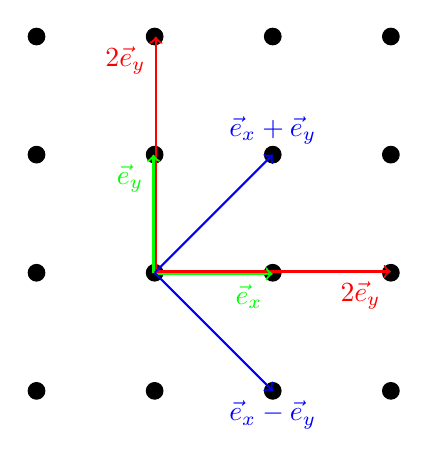
\begin{tikzpicture}[scale=1.5]
 \foreach \x in {1,...,4}
 \foreach \y in {1,...,4}
 \filldraw  (\x,\y) circle (2pt);
 \draw[->,red  ,thick] (2.01,2) -- (2.01,4) node[anchor=north east] {$2\vec e_y$};
 \draw[->,red  ,thick] (2,2.01) -- (4,2.01) node[anchor=north east] {$2\vec e_y$};
 \draw[->,green,thick] (1.99,2) -- (1.99,3) node[anchor=north east] {$\vec e_y$};
 \draw[->,green,thick] (2,1.99) -- (3,1.99) node[anchor=north east] {$\vec e_x$};
 \draw[->,blue ,thick] (2,2) -- (3,3) node[anchor= south] {$\vec e_x+ \vec e_y$};
 \draw[->,blue ,thick] (2,2) -- (3,1) node[anchor=north ] {$\vec e_x- \vec e_y$}; 
 \end{tikzpicture}
\end{center}
\caption{Translation vectors $\vec T_d$ in a two dimensional square lattice for first (green), second (blue) and third (red) neighbour interactions.}
\label{2d_square}
\end{figure}

The additional term one gets for non-zero second and third neighbour interactions can be treated the same way. 
One has to include the corresponding translational vectors $\vec T_d$ with their respective couplings.
Figure \ref{2d_square} shows the vectors up to third neighbour interactions in the 2D square lattice.
The third neighbours have the same type of translational vectors as the first neighbours, just with twice the length.
The second neighbours are found at $\vec e_x \pm \vec e_y$.
The resulting expression for the energy dispersion in this situation reads
\begin{equation}
 \varepsilon_{\vec k } = -2t \left(\cos k_x + \cos k_y \right) -4t^{\prime} \cos k_x \cos k_y  -2t^{\prime \prime} \left( \cos 2k_x + \cos 2k_y \right)
\end{equation}

We note that the hopping term represents the kinetic energy of particles moving between different sites. 
It is the hopping parameter and the 
geometry of the lattice, that provide the energy dispersion. 
The energy dispersion for Sr$_2$IrO$_4$  with and without next-to-nearest neighbour interactions are shown in figure \ref{fig:energie_dispersion}.



\begin{figure} \centering
\begin{subfigure}{0.49\linewidth} \centering
 \includegraphics[width=\textwidth]{../tBandstructure}
 \caption{$ t^{\prime}=t^{\prime \prime} =0$ }
\end{subfigure}
\begin{subfigure}{0.49\linewidth}
\includegraphics[width=\textwidth]{../tttBandstructure}
  \caption{ $t^{\prime}= 0.2326t$, $t^{\prime \prime} = 0.1163t$}
\end{subfigure}
\caption{
Contour plots of the single particle energy dispersion in units of t. Momenta are given in units of $2\pi$.
The arrow is a vector, called the nesting vector $\vec Q$, that connects large parts of the
Fermi surface. This symmetry leads to an anti-ferromagnetic ground state.}
\label{fig:energie_dispersion}
\end{figure}




\subsection{Hubbard Interaction}

So far we did not take any interactions between particles into account.
The general form of a two particle operator is
\begin{equation}
 H_{\text{int}} = \sum_{\sigma_1 \sigma_2 \sigma_3 \sigma_4} \; \sum_{ijkl} U_{ijkl} \, c^{\dagger}_{i,\sigma_1} c^{\dagger}_{j,\sigma_2} c_{k,\sigma_3} c_{l,\sigma_4}
\end{equation}
%
The matrix elements $U_{ijkl}$ are independent of spin and given by
\begin{equation}
 U_{ijkl} = \int \!  \dint^3 r  \, \dint^3 r^{\prime} \,  \varphi_i^*(\vec{r}) \varphi_j^*(\vec{r}^{\prime}) \frac{e^2}{|\vec{r}-\vec{r}^{\prime} |} \varphi_k(\vec{r}) \varphi_l(\vec{r}) 
\end{equation}
Due to the small overlap of different states $\varphi_i$, only a few matrix elements are important.
The diagonal matrix elements $U_{iiii} = U$ account for the repulsion between electrons on the same site and are certainly the most important contribution.
%
From the fermionic commutation relations we know that $c^{\dagger 2}_{\vec k,\sigma}=c_{\vec k,\sigma}^2=0$.
The only non-zero term proportional to $U_{iiii}$ is therefore $c^{\dagger}_{i,\uparrow} c^{\dagger}_{i,\downarrow} c_{i,\uparrow} c_{i,\downarrow}$. 
Using the number operator $n_{i,\sigma} = c^{\dagger}_{i,\sigma} c_{i,\sigma}$, the diagonal interaction term reads
\begin{equation}
 H_{\text{int}} = U \sum_i n_{i,\uparrow} n_{i,\downarrow}.
\end{equation}
Other terms count the interaction of density fluctuations at neighbouring sites through $U_{ijij}$ 
or
the exchange coupling $U_{ijji}$, which yields a Heisenberg like coupling $J_{ij}$.

In the Hubbard model however we take only the diagonal terms $U_{iiii}$ into account.
We choose therefore $U_{ijkl} = \delta_{ijkl} U$. 
Reducing an interaction that is not necessarily local to only on-site interactions is a grave simplification, 
neglecting the vast amount of parameters in the interaction matrix $U_{ijkl}$ and therefore long range repulsion and exchange effects.
As a result, the optimal value for $U$, the only parameter left, does not any longer depend on the integral given above in a simple way.
The interaction seems to be drastically lowered due to screening effects compared to the value one would expect from the correlation integral of the corresponding orbitals
\cite{J.Phys.Cond.Matter.Vol21.34}.
It is not possible to link the parameter $U$ to a physical quantity directly
and the Hubbard model is therefore not a first principle model. 
$U$ will be treated as an effective parameter and chosen in order to describe the observed behaviour correctly. 



% Mott Insulator (band split-up using U)
% How U changes the picture


%The Hubbard model is defined by the Hamiltonian
%\begin{equation}
% \hat{H} = \hat{H}_0
%	   + U \sum_i c^{\dagger}_{i,\uparrow}c_{i,\uparrow} c^{\dagger}_{i,\downarrow}c_{i,\downarrow} 
%	    . \label{Hubbard_space}
%\end{equation}
%with a band structure single particle Hamiltonian $\hat{H}_0$.

\subsubsection{Hubbard Term In Momentum Space}

We can express the interaction term through creation and annihilation operators in momentum space as well. 
The summation over all sites in the transformation yields an overall $\delta$-function of momenta,
\begin{IEEEeqnarray}{rl}
 &\frac{U}{N^2} \sum_{\vec{k}\vec{l}\vec{m}\vec{n}} \sum_i \euler^{-\im (\vec{k}-\vec{l}+\vec{m}-\vec{n})\vec{R}_i } 
    c^{\dagger}_{\vec{k},\uparrow}c_{\vec{l},\uparrow} c^{\dagger}_{\vec{m},\downarrow}c_{\vec{n},\downarrow} \nonumber \\
    =& \frac{U}{N} \sum_{\vec{k}\vec{l}\vec{m}\vec{n}} \delta(\vec{k}-\vec{l}+\vec{m}-\vec{n} )
	c^{\dagger}_{\vec{k},\uparrow}c_{\vec{l},\uparrow} c^{\dagger}_{\vec{m},\downarrow}c_{\vec{n},\downarrow} \nonumber \\
    =& \frac{U}{N} \sum_{\vec{k}\vec{k}^{\prime}\vec{q}}
	c^{\dagger}_{\vec{k},\uparrow}c_{\vec{k}-\vec{q},\uparrow} c^{\dagger}_{\vec{k}^{\prime},\downarrow}c_{\vec{k}^{\prime}+\vec{q},\downarrow} \:.
 \end{IEEEeqnarray}
In the last line we choose a convenient parametrization of momenta. 
The interaction is non-diagonal, but it ensures momentum conversation at each vertex.

The total expression for the Hamiltonian in momentum space reads
 \begin{equation}
  \hat{H} = \sum_{\vec{k},\sigma} \left(\varepsilon_{\vec k} - \mu\right) c^{\dagger}_{\vec{k},\sigma}c_{\vec{k},\sigma} + \frac{U}{N} \sum_{\vec{k}\vec{k}^{\prime}\vec{q}}
	c^{\dagger}_{\vec{k},\uparrow}c_{\vec{k}-\vec{q},\uparrow} c^{\dagger}_{\vec{k}^{\prime},\downarrow}c_{\vec{k}^{\prime}+\vec{q},\downarrow}
 \end{equation} 


